
Composing CMake code is very much like writing in any other imperative language: lines are executed from top to bottom and from left to right, occasionally stepping into an included file or a called function. Depending on the mode (see the Mastering the command line section in Chapter 1, First Steps with CMake), the execution begins from the root file of the source tree (CMakeLists.txt) or a .cmake script file that was passed as an argument to cmake.

As we discussed in the previous chapter, scripts support the majority of the CMake Language (with the exclusion of any project-related functionality). As a result, they're a great way to start practicing the CMake syntax itself, and that's why we'll be using them here. After becoming comfortable writing basic listfiles, we'll start preparing actual project files in the next chapter. If you remember, scripts can be run with the following command:

\begin{tcblisting}{commandshell={}}
cmake -P script.cmake
\end{tcblisting}

\begin{tcolorbox}[colback=blue!5!white,colframe=blue!75!black,title=Note]
CMake supports 7-bit ASCII text files for portability across all platforms. You can use both \verb|\|n or \verb|\|r\verb|\|n line endings. UTF-8 with optional Byte Order Markers (BOMs) is supported in CMake versions above 3.0, and UTF-16 is supported in CMake versions above 3.2.
\end{tcolorbox}

Everything in a CMake listfile is either a command invocation or a comment.

\subsubsubsection{2.2.1\hspace{0.2cm}Comments}

Just like in C++, there are two kinds of comments – single-line comments and bracket (multiline) comments. But unlike in C++, bracket comments can be nested. Let me show you the syntax:

\begin{lstlisting}[style=styleCMake]	
# single-line comments start with a hash sign "#"
# they can be placed on an empty line
message("Hi"); # or after a command like here.

#[=[
bracket comment
	#[[
		nested bracket comment
	#]]
#]=]
\end{lstlisting}

Multiline comments get their name from their symbol – they start with an opening square bracket ([), any number of equal (=) signs, and another square bracket: [=[. To close a bracket comment, use the same number of equal signs and reverse the brackets like so: ]=].

Prepending opening bracket tokens with \# is optional, and allows you to quickly disable a multiline comment by adding another \# to the first line of the bracket comment like so:

\begin{lstlisting}[style=styleCMake]	
##[=[ this is a single-line comment now
no longer commented
	#[[
		still, a nested comment
	#]]
#]=] this is a single-line comment now
\end{lstlisting}

That's a nifty trick, but when and how should we use comments in our CMake file? Since writing listfiles is essentially programming, it is a good idea to bring our best coding practices to them as well. Code that follows such practices is often called clean – a term used over the years by software development gurus like Robert C. Martin, Martin Fowler, and many other authors. What's considered helpful and harmful is often heavily disputed and, as you might guess, comments have not been left out of these debates.

Everything should be judged on a case-by-case basis, but generally agreed-upon guidelines say that good comments provide at least one of the following:

\begin{itemize}
\item 
Information: They can untangle complexities such as regex patterns or formatting strings.

\item 
Intent: They can explain the intent of the code when it is unobvious from the implementation or interface.

\item 
Clarification: They can explain concepts that can't be easily refactored or changed.

\item 
Warnings of consequences: They can provide warnings, especially around code that can break other things.

\item 
Amplification: They can underline the importance of an idea that is hard to express in code.

\item 
Legal clauses: They can add this necessary evi, which is usually not the domain of a programmer.
\end{itemize}

If you can, avoid adding comments and adopt better naming practices, or refactor or correct your code. If you can, avoid adding comments of the following types:

\begin{itemize}
\item 
Mandated: These are added for completeness, but they are not really important.

\item 
Redundant: These repeat what is already clearly written in the code.

\item 
Misleading: These could be outdated or incorrect if they don't follow code changes.

\item 
Journal: These note what has been changed and when (use VCS for this instead).

\item 
Dividers: These mark sections.
\end{itemize}

Writing elegant code without comments is hard, but it improves the experience of the reader. Since we spend more time reading code than writing it, we should always try to write readable code, instead of just trying to write it quickly. I recommend checking out the Further reading section at the end of this chapter for some good references on clean code. If you're interested in comments in particular, you'll find a link to one of my many YouTube videos touching on this subject in depth.


\subsubsubsection{2.2.2\hspace{0.2cm}Command invocations}

Time for some action! Invoking commands is the bread and butter of CMake listfiles. To execute a command, you must provide its name, followed by parentheses, in which you may enclose a whitespace-separated list of command arguments.

\begin{center}
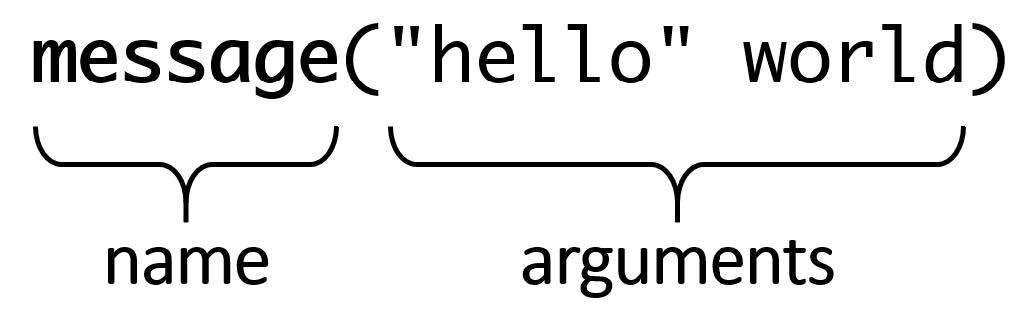
\includegraphics[width=0.5\textwidth]{content/1/chapter2/images/1.jpg}\\
Figure 2.1 – An example of a command
\end{center}

Command names aren't case-sensitive, but there is a convention in the CMake community to use snake\_case in command names (that is, lower-case words joined with underscores).
You can also define your own commands, which we'll cover in the Understanding control structures in CMake section of this chapter.

What's especially striking in comparison to C++ is the fact that command invocations in CMake are not expressions. You can't provide another command as an argument to a called command, as everything between the parentheses is interpreted as an argument for that command.

Even more enraging is the fact that CMake commands don't require semicolons at the end of an invocation. This may be because each line of source can contain up to one command invocation, followed by an optional single-line comment. Alternatively, an entire line has to be part of a bracket comment. So, these are the only allowed formats:

\begin{lstlisting}[style=styleCMake]	
command(argument1 "argument2" argument3) # comment
[[ multiline comment ]]
\end{lstlisting}

Putting a command after a bracket comment is not allowed:

\begin{lstlisting}[style=styleCMake]	
[[ bracket
]] command()
\end{lstlisting}

After removing any comments, whitespace, and empty lines, we get a list of command invocations. This creates an interesting perspective – CMake syntax is really simple, but is that a good thing? How do we even work with variables? Or, how do we direct the flow of the execution?

CMake provides commands for these actions and much more. To make things easier, we'll be introducing the relevant commands as we move through different examples, and they can be grouped into three categories:

\begin{itemize}
\item 
Scripting commands: These are always available, and they change the state of the command processor, access variables, and affect other commands and the environment.

\item 
Project commands: These are available in projects, and they manipulate the project state and build targets.

\item 
CTest commands: These are available in CTest scripts. They manage testing.
\end{itemize}

We'll cover the most useful scripting commands in this chapter (as they are also useful in projects). Project and CTest commands will be discussed in the following chapters as we introduce the concepts relating to build targets (Chapter 3, Setting Up Your First CMake Project) and testing frameworks (Chapter 8, Testing Frameworks).

Virtually every command relies on other elements of the language in order to function: variables, conditional statements, and first and foremost, command-line arguments. Let's see how we should use these.

\subsubsubsection{2.2.3\hspace{0.2cm}Command arguments}

Many commands require whitespace-separated arguments to parametrize how they behave. As you saw in Figure 2.1, there's something weird happening with the quotes around the arguments. Some arguments have quotes and others don't – what's up with that?

Under the hood, the only data type recognized by CMake is a string. This is why every command expects zero or more strings for its arguments. But plain, static strings aren't very useful, especially when we can't nest command invocations. Here's where arguments come into play – CMake will evaluate every argument to a static string and then pass them into the command. Evaluating means string interpolation, or substituting parts of a string with another value. This can mean replacing the escape sequences, expanding the variable references (also called variable interpolation), and unpacking lists.

Depending on the context, we might want to enable such evaluation as needed. And for that reason, CMake offers three types of arguments:

\begin{itemize}
\item 
Bracket arguments

\item 
Quoted arguments

\item 
Unquoted arguments
\end{itemize}

Each argument type offers a different level of evaluation and has a few small quirks to it.

\hspace*{\fill} \\ %插入空行
\noindent
\textbf{Bracket arguments}

Bracket arguments aren't evaluated because they are used to pass multiline strings, verbatim, as a single argument to commands. This means it will include whitespace in the form of tabs and newlines.

These arguments are structured exactly like comments – that is, they are opened with [=[ and closed with ]=], where the number of the equal signs in the opening and closing tokens has to match (skipping the equal signs is fine too, but they still have to match). The only difference from comments is that you can't nest bracket arguments.

Here's an example of the use of such an argument with the message() command, which prints all passed arguments to the screen:

\begin{lstlisting}[style=styleCMake]
# chapter02/01-arguments/bracket.cmake	

message([[multiline
bracket
argument
]])

message([==[
	because we used two equal-signs "=="
	following is still a single argument:
	{ "petsArray" = [["mouse","cat"],["dog"]] }
]==])
\end{lstlisting}

In the above example, we can see different forms of bracket arguments. The first one skips the equal sign. Note how putting closing tags on a separate line is visible as an empty line in the output:

\begin{tcblisting}{commandshell={}}
$ cmake -P chapter02/01-arguments/bracket.cmake
multiline
bracket
argument

  because we used two equal-signs "=="
  following is still a single argument:
  { "petsArray" = [["mouse","cat"],["dog"]] }
\end{tcblisting}

The second form is useful when we're passing text that contains double brackets (]]) (highlighted in the code snippet), as they won't be interpreted as marking the end of the argument.

These kinds of bracket arguments have limited use – typically, to contain longer blocks of text. In most cases, we'll need something more dynamic, such as quoted arguments.

\hspace*{\fill} \\ %插入空行
\noindent
\textbf{Quoted arguments}

Quoted arguments resemble a regular C++ string – these arguments group together multiple characters, including whitespace, and they will expand escape sequences. Like C++ strings, they are opened and closed with a double quote character ("), so to include a quote character within the output string, you have to escape it with a backslash (\verb|\|").

Other well-known escape sequences are supported as well: \verb|\|\verb|\| denotes a literal backslash, \verb|\|t is a tab character, \verb|\|n is a newline, and \verb|\|r is a carriage return.

This is where the similarities with C++ strings end. Quoted arguments can span multiple lines, and they will interpolate variable references. Think of them as having a built-in sprintf function from C or a std::format function from C++20. To insert a variable reference to your argument, wrap the name of the variable in a token like so: \$\{name\}.

We'll talk more about variable references in the Working with variables section.
Let's try these arguments in action:

\begin{lstlisting}[style=styleCMake]
# chapter02/01-arguments/quoted.cmake
	
message("1. escape sequence: \" \n in a quoted argument")
message("2. multi...
	line")
message("3. and a variable reference: ${CMAKE_VERSION}")
\end{lstlisting}

Can you guess how many lines will be in the output of the preceding script?

\begin{tcblisting}{commandshell={}}
$ cmake -P chapter02/01-arguments/quoted.cmake
1. escape sequence: "
 in a quoted argument
2. multi...
line
3. and a variable reference: 3.16.3
\end{tcblisting}

That's right – we have one escaped quote character, one escaped newline, and a literal newline. All of them will be printed in the output. We also accessed a built-in CMAKE\_VERSION variable, which we can see correctly interpolated on the last line.

\hspace*{\fill} \\ %插入空行
\noindent
\textbf{Unquoted arguments}

The last type of argument is definitely a bit rare in the programming world. We got used to the fact that strings have to be delimited in one way or another, for example, by using single quotes, double quotes, or a backslash. CMake deviates from this convention and introduces unquoted arguments. We might argue that dropping delimiters makes the code easier to read, just like skipping semicolons. Is that true? I'll let you form your own opinion.

Unquoted arguments evaluate both escape sequences and variable references. However, be careful with semicolons (;), as in CMake, this is treated as a delimiter. CMake will split the argument containing it into multiple arguments. If you need to use it, escape it with a backslash (\verb|\|;). This is how CMake manages lists. I'll explain that in detail in the Using lists section.

You may find that these arguments are the most perplexing to work with, so here's an illustration to help clarify how these arguments are partitioned:

\begin{center}
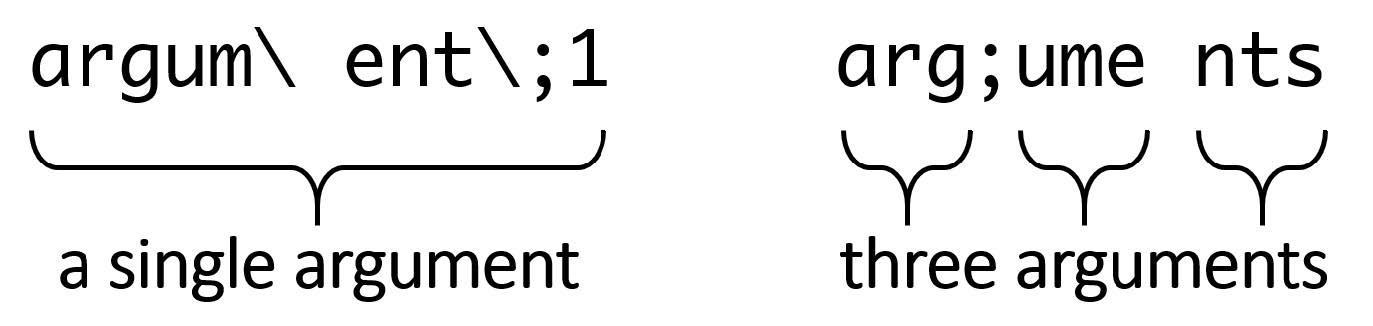
\includegraphics[width=0.5\textwidth]{content/1/chapter2/images/2.jpg}\\
Figure 2.2 – Escape sequences cause separate tokens to be interpreted as a single argument
\end{center}

\begin{tcolorbox}[colback=black!5!white,colframe=black!75!black,title=Question]
Why does it matter if a value is passed as a single argument or many arguments? Some CMake commands require a specific number of arguments and ignore any overhead. If your arguments accidentally become separated, you'll get hard-to-debug errors.
\end{tcolorbox}

Unquoted arguments cannot contain unescaped quotes ("), hashes (\#), and backslashes (\verb|\|). And if that's not enough rules to remember, parentheses (()) are allowed only if they form correct, matching pairs. That is, you'll start with an opening parenthesis and close it before closing the command argument list.

Let's look at some examples of all of the above rules:

\begin{lstlisting}[style=styleCMake]
# chapter02/01-arguments/unquoted.cmake
	
message(a\ single\ argument)
message(two arguments)
message(three;separated;arguments)
message(${CMAKE_VERSION}) # a variable reference
message(()()()) # matching parentheses
\end{lstlisting}

What will be the output of the above? Let's have a look:

\begin{tcblisting}{commandshell={}}
$ cmake -P chapter02/01-arguments/unquoted.cmake
a single argument
twoarguments
threeseparatedarguments
3.16.3
()()()
\end{tcblisting}

Even a simple command such as message() is very particular about separated unquoted arguments:

\begin{itemize}
\item 
The space in a single argument was correctly printed when it was explicitly escaped.

\item 
However, twoarguments and threeseparatearguments were glued together, since message() doesn't add any spaces on its own.
\end{itemize}

Now that we understand how to deal with the complexities and quirks of CMake arguments, we are ready to tackle the next interesting subject – working with all kinds of variables in CMake.









